% 2010 年重庆卷文科第 15 题：由三段圆弧连接而成的封闭曲线 C。
% 来源 PDF：普通高考/2010/2010重庆文.pdf，SHA-256 634c8ac529a6ea52305b2909eff8730888048b77d082897394bfda22cb3fe73b。
% 原页：第 1 页（A3 三栏）第 2 栏中部，书页码 579。
% 重绘依据：原页三个等半径圆两两相交，三圆都经过同一点 P（图中实心点），
%   左侧、右侧、下方各一个圆；封闭曲线 C 由三圆的外侧弧（实线）连接而成，
%   含 P 的内侧弧在原页为虚线，此图照录。
% 原页三圆心近似成等边三角形分布，这里按题面「半径相等」取理想位置：三圆心在
%   以 P 为心、半径 r=1 的圆上，方向角 150°、30°、270°；三段外弧圆心角均为 240°。
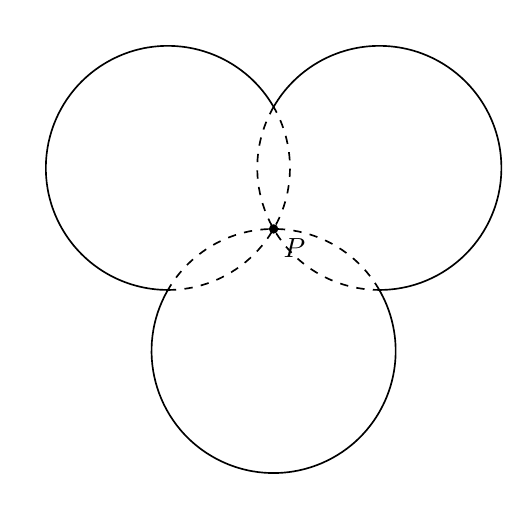
\begin{tikzpicture}[scale=1.55, semithick]
  \coordinate (P) at (0,0);
  \coordinate (O1) at (-0.8660254,0.5);
  \coordinate (O2) at (0.8660254,0.5);
  \coordinate (O3) at (0,-1);

  % 封闭曲线 C：三段不含 P 的外侧弧（实线）
  \draw (O1) ++(30:1) arc[start angle=30, end angle=270, radius=1];
  \draw (O2) ++(-90:1) arc[start angle=-90, end angle=150, radius=1];
  \draw (O3) ++(150:1) arc[start angle=150, end angle=390, radius=1];

  % 三个圆上含 P 的内侧弧（原页虚线）
  \draw[dashed] (O1) ++(270:1) arc[start angle=270, end angle=390, radius=1];
  \draw[dashed] (O2) ++(150:1) arc[start angle=150, end angle=270, radius=1];
  \draw[dashed] (O3) ++(30:1) arc[start angle=30, end angle=150, radius=1];

  % 公共点 P 及标注
  \fill (P) circle (1.1pt);
  \node[below right] at (P) {$P$};
\end{tikzpicture}
